\section{Thesis outline}
% \todo{Making key word cursive, like persistence length, SSDNA 1, ...}

All organisms in nature tirelessly perform work, struggling against an ever increasing
entropy. This work is collectively performed by a countless number of molecular machines,
all contributing to their specific tasks.

Despite being so abundantly present in nature, fabricating synthetic molecular machines
turns out to be a difficult task. One of the biggest hurdles in this process arises from
their corresponding length-scale. Often times these machines are not larger then
a few nanometres, making the typical energy associated with the bonds and
distortions of their structure comparable to thermal energy fluctuations. As a result of
these thermal fluctuations in their environment molecular machines naturally perform
a stochastic motion that complicates their functioning.  Extracting useful work from
these freely tumbling structures is almost impossible. To overcome this limitation most
synthetic molecular machines are embedded in a larger complex providing necessary
stability.\cite{Watson2016}

This phenomenon is also observed in nature, for instance in the interfacing of protein
complexes with the phospholipid bilayer of cells.  A wildly known example is the
bacterial flagella motor, which provides an efficient way for bacteria to
roll and tumble throughout their environment. Just like in electrical motors, the
flagella consists of a stator and a rotor. The stator is anchored into the cell membrane,
while the rotor is allowed to freely rotate. The work is produced by the flow of cations
through the stator. Inducing changes in the electrostatic interactions between the two
parts of the flagella generates a unidirectional motion.\cite{sowa_berry_2008}\\

Similarly to macroscopic engines, heat is produced during the operation of molecular
machines. When the structure is not capable of dissipating this heat efficiently, an
excessive build-up compromises its durability. To mitigate this problem, large and soft
molecules are often used in the design of nanomachines. A logical choice
is the use of polymers, which can effectively dissipate heat as a result of their
flexibility.  Due to the programmability of DNA, using the Watson-Crick interactions,
the DNA polymer provides additional aptitude. This makes DNA a popular material in
nanotechnology.

The central topic of this thesis is studying the DNA nanopiston (Bayoumi et
al.\cite{Bayoumi21}), a DNA based molecular machine embedded into a phospholipid
membrane. This
nanopiston can be characterised as an autonomous molecular machine, which turns over
chemical fuel to continuously perform work. The aim of this complex is to perform
selective transport of DNA through a membrane.

The operation cycle of previously designed DNA transporters requires a supporting
external bias.\cite{Franceschini2013} However, this specific nanopiston operates also
against an external bias. The physics driving this machine is entropy and will be
discussed in detail in throughout this thesis.

In the first chapter a comprehensive introduction of important concepts
regarding the DNA nanopiston is given. Having laid this theoretical foundation, the
structure and operation cycle of the DNA nanopiston is discussed in chapter two. Next the
computational model used in this thesis is presented in chapter three. In chapter four,
the results of these simulations is discussed. Finally chapter five will offer a
discussion of these results and recommendations for further research.
\vspace{0.5cm}
\begin{figure}[ht]
\begin{center}
  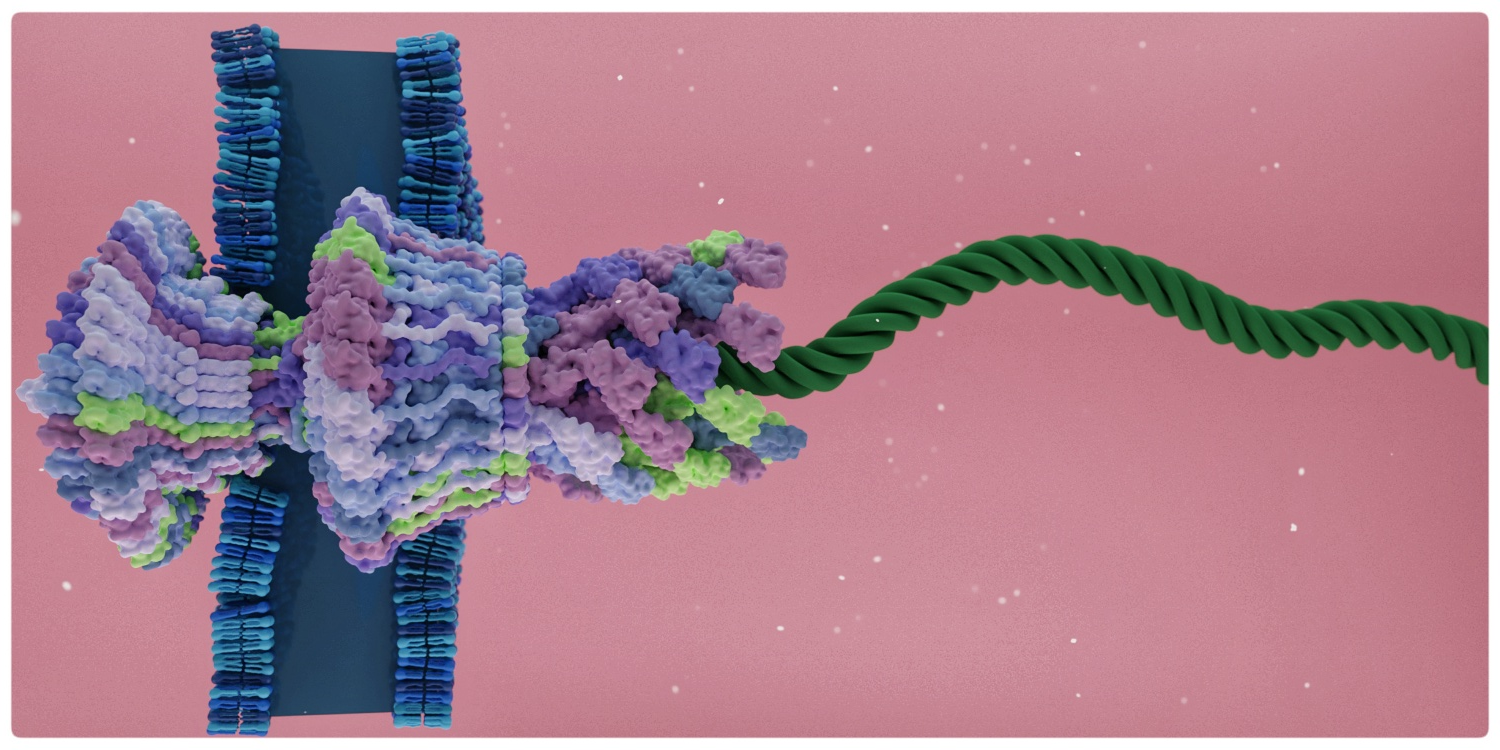
\includegraphics[width=0.85\textwidth]{Figures/flagella2.png}
  \caption{Flagella motor, cite pdb paper, chimera and blender!}
\end{center}
\end{figure}
